% ============================================================================
\section{Preliminaries}
\label{sec:preliminaries}
% ============================================================================

Let $G$ be a (not necessarily simple) \emph{topological graph}, that is, $G$ is a graph drawn on the plane, so that the vertices of $G$ are distinct points in the plane, its edges are Jordan courves joining the corresponding pairs of points, and:%
%
\begin{inparaenum}[(i)]
\item no edge passes through a vertex different from its endpoints, 
\item no edge crosses itself and 
\item no two edges meet tangentially.
\end{inparaenum}
Let $\Gamma(G)$ be such a drawing of $G$. The \emph{crossing graph} $\mathcal{X}(G)$ of $G$ has a vertex for each edge of~$G$, while two vertices of $\mathcal{X}(G)$ are connected by an edge if and only if the corresponding edges of $G$ cross in $\Gamma(G)$. A connected component of $\mathcal{X}(G)$ is called \emph{crossing component}. Observe that the set of crossing components of $\mathcal{X}(G)$ define a partition of the edges $G$. Given an edge $e$ of $G$ we denote by $\mathcal{X}(e)$ the crossing component of $\mathcal{X}(G)$ which contains $e$. 

An edge $e$ in $\Gamma(G)$ is called a \emph{topological edge} (or simply edge, if this is clear in the context). Edge $e$ is called \emph{true-planar}, if it is not crossed by any other edge in $\Gamma(G)$. The set of all true-planar edges of $\Gamma(G)$ forms the so-called \emph{true-planar skeleton} of $\Gamma(G)$, which we denote by $\Pi(G)$. Since $G$ is not necessarily simple, we will further assume that $\Gamma(G)$ contains neither \emph{homotopic parallel edges} nor \emph{homotopic self-loops}, that is, both the interior and the exterior regions defined by any self-loop or by any pair of parallel edges contain at least one vertex. For a possitive integer $s$, a cycle of length $s$ is called \emph{true-planar $s$-cycle} if it consists of true-planar edges of $\Gamma(G)$. Clearly, if $e$ is a true-planar edge, then $\mathcal{X}(e)=\{e\}$, while for a chord $e$ of a true-planar $s$-cycle that has no vertices in its interior, it follows that all edges of $\mathcal{X}(e)$ are also chords of this $s$-cycle. Let $\mathcal{F}_s=\{v_1,v_2,\ldots,v_s\}$ be a facial $s$-cycle of $\Pi(G)$ with length $s \geq 3$.  The order of the vertices (and subsequently the order of the edges) of $\mathcal{F}_s$ is determined by a walk around the boundary of $\mathcal{F}_s$ in clockwise direction. Since $\mathcal{F}_s$ is not necessarily simple, a vertex (or an edge, respectively) may appear more than once in this order; see Figure~\ref{fig:non_simple_face}.

\begin{figure}[tb]
    \centering	
	\begin{minipage}[b]{.18\textwidth}
        \centering
        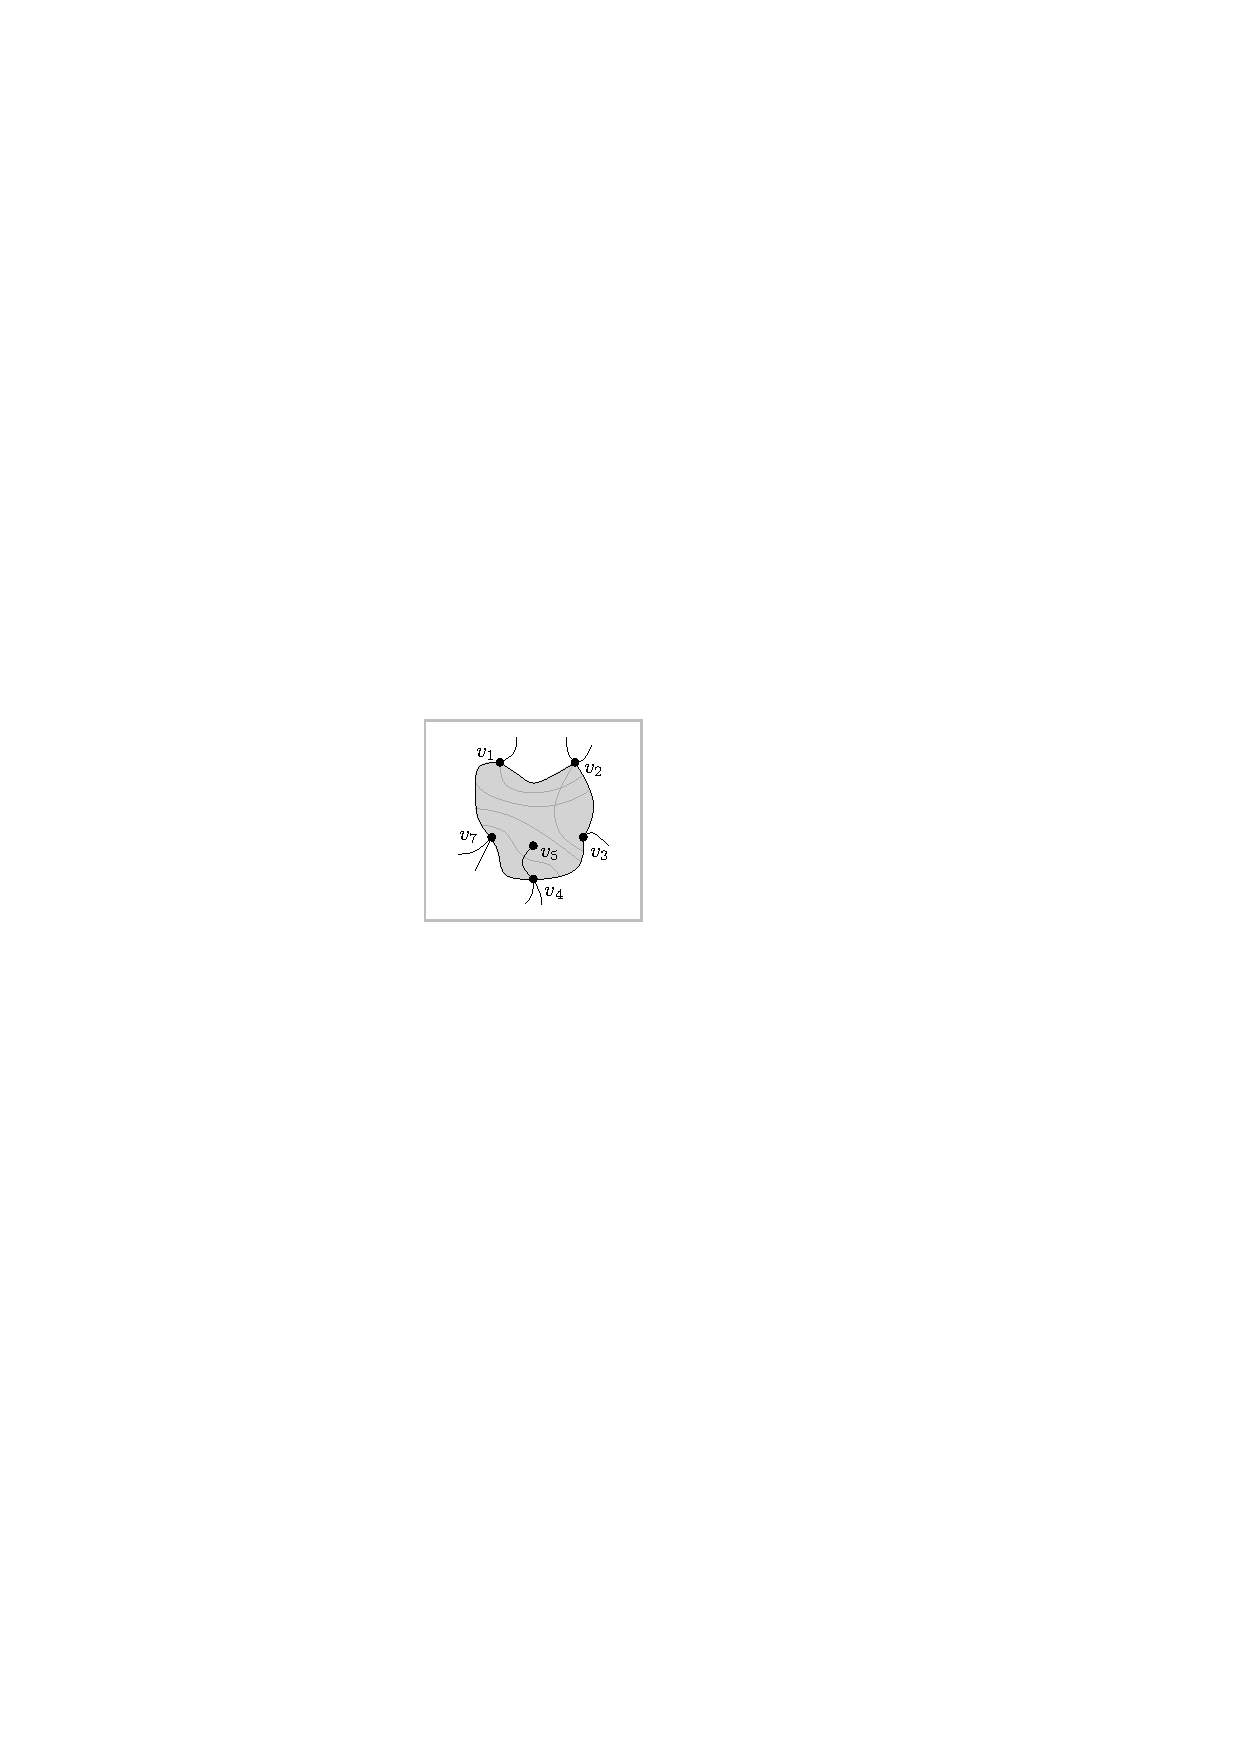
\includegraphics[width=\textwidth,page=1]{images/preliminaries}
        \subcaption{~}\label{fig:non_simple_face}
    \end{minipage}
	\begin{minipage}[b]{.18\textwidth}
        \centering
        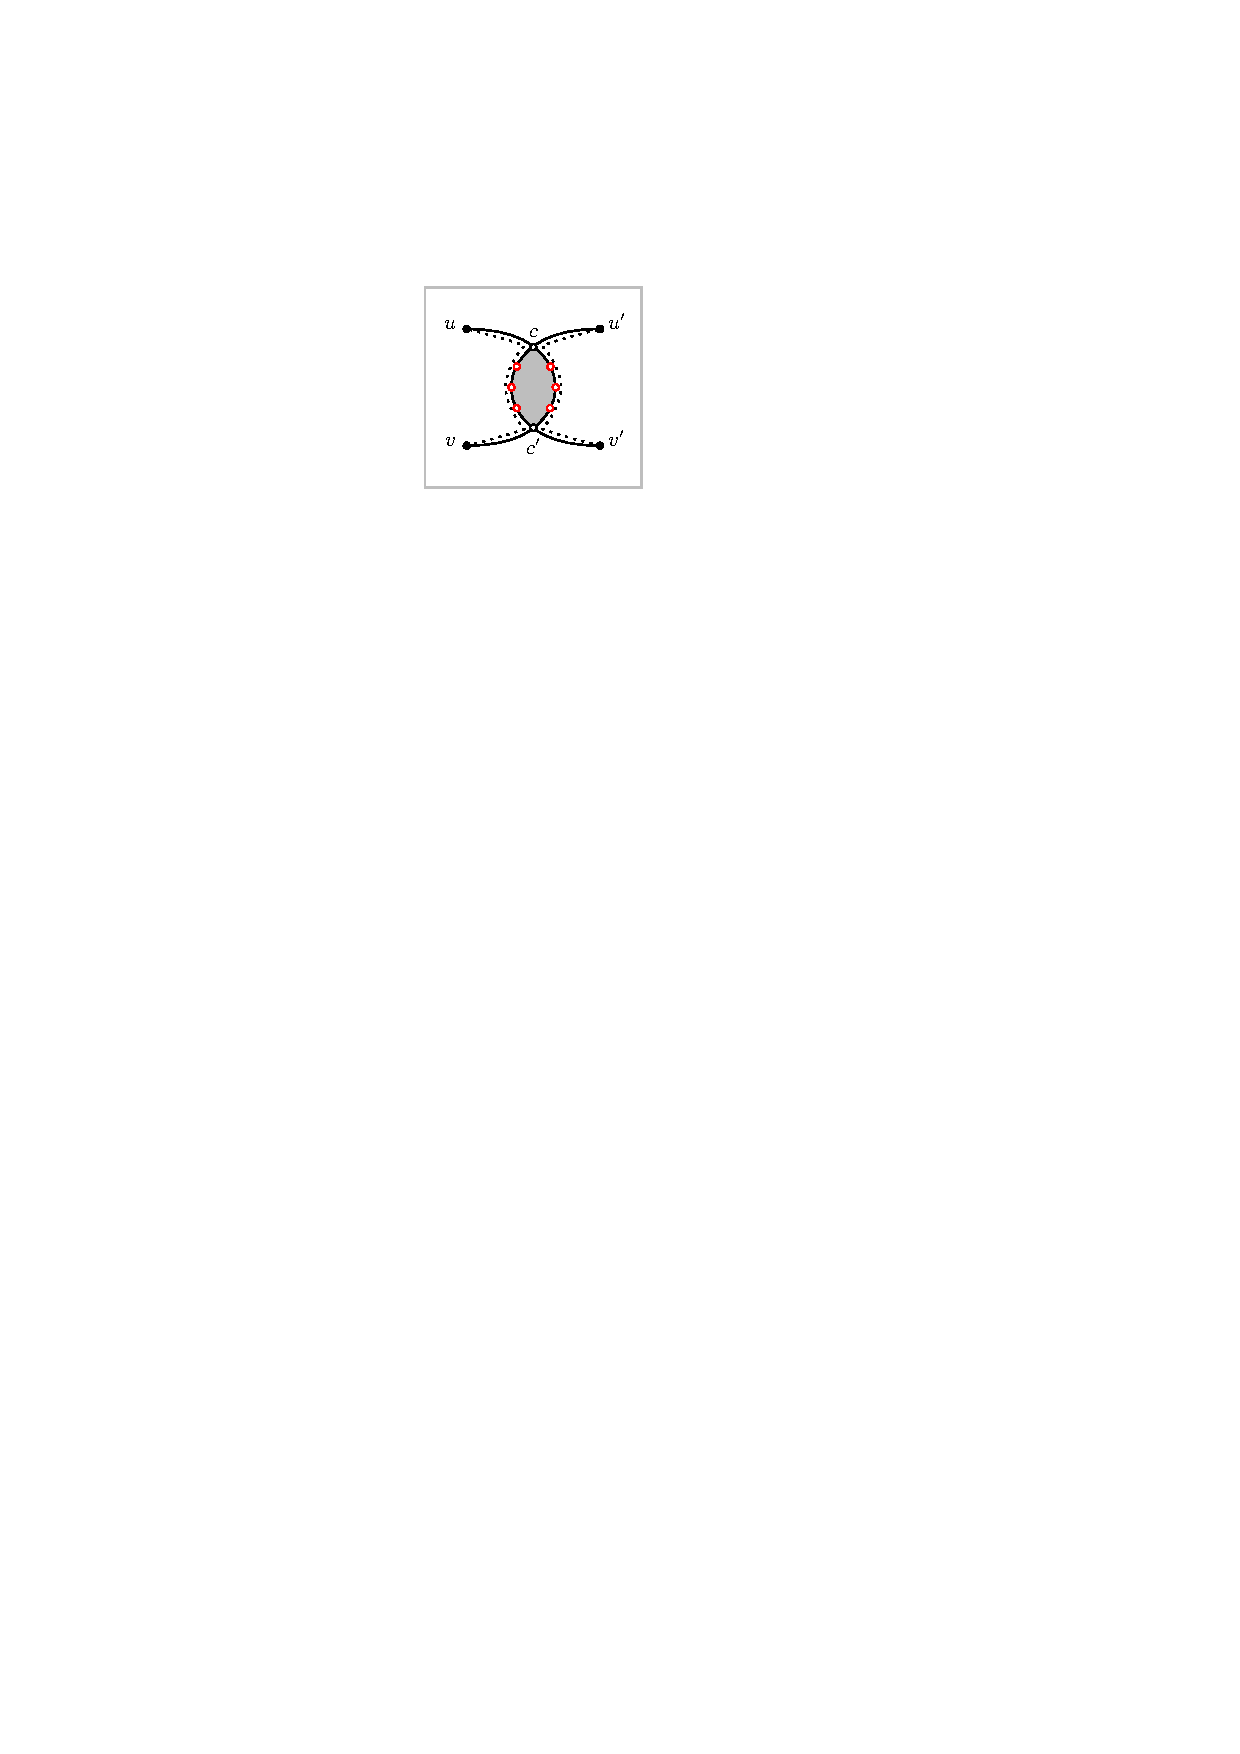
\includegraphics[width=\textwidth,page=1]{images/crossing_conf}
        \subcaption{~}\label{fig:crossing_twice}
    \end{minipage}	
    \begin{minipage}[b]{.18\textwidth}
        \centering
        \includegraphics[width=\textwidth,page=2]{images/crossing_conf}
        \subcaption{~}\label{fig:crossing_twice_2}
    \end{minipage}
    \begin{minipage}[b]{.18\textwidth}
        \centering
        \includegraphics[width=\textwidth,page=3]{images/crossing_conf}
        \subcaption{~}\label{fig:crossing_adjacent}
    \end{minipage}	
    \begin{minipage}[b]{.18\textwidth}
        \centering
        \includegraphics[width=\textwidth,page=4]{images/crossing_conf}
        \subcaption{~}\label{fig:crossing_adjacent_2}
    \end{minipage}	
    \caption{%
    (a)~A non-simple face $\{v_1,\ldots,v_7\}$, where $v_6$ is identified with $v_4$.
    Different configurations used in 
    (b-c)~Lemma~\ref{lem:crossing_twice}, and 
    (d-e)~Lemma~\ref{lem:crossing_adjacent}.}
    \label{fig:2_planar_polygon_conf}
\end{figure} 

Drawing $\Gamma(G)$ is called \emph{$k$-planar} if every edge in $\Gamma(G)$ is crossed at most $k$ times. Accordingly, a graph is called \emph{$k$-planar} if it admits a $k$-planar drawing. An \emph{optimal $k$-planar} graph is a $k$-planar graph with the maximum number of edges (e.g., an optimal $1$-planar graph on $n$ vertices is a $1$-planar graph with exactly $4n-8$ edges). For an optimal $k$-planar graph $G$ on $n$ vertices, a $k$-planar drawing $\Gamma(G)$ of $G$ is called \emph{planar-maximal crossing-minimal} or simply PMCM-drawing if and only if $\Gamma(G)$ has the maximum number of true-planar edges among all $k$-planar drawings of $G$ and, subject to this restriction, $\Gamma(G)$ has also the minimum number of crossings.

\begin{lemma}
Let $\Gamma(G)$ be a PMCM-drawing of an optimal $k$-planar graph $G$ in which two edges $(u,v)$ and $(u',v')$ cross more that once. Let $c$ and $c'$ be two consecutive crossing points along $(u,v)$. Then, the closed region $R_{c,c'}$ that is defined by the edge segments of $(u,v)$ and $(u',v')$ between $c$ and $c'$ has at least one vertex in its interior.
\label{lem:crossing_twice}
\end{lemma}
\begin{proof}
For a proof by contradiction, assume that there is no vertex in $R_{c,c'}$. Denote by $nc(u,v)$ and $nc(u',v')$ the number of crossings along $(u,v)$ and $(u',v')$ that are between $c$ and $c'$, respectively (red drawn in Figure~\ref{fig:crossing_twice}). First assume that $nc(u,v) = nc(u',v')$. We will cope with the case where $nc(u,v) \neq nc(u',v')$ shortly. We proceed by redrawing edge $(u,v)$ and $(u',v')$ so to eliminate both crossings $c$ and $c'$ without affecting the $k$-planarity of $G$; see the dotted-drawn edges of Figure~\ref{fig:crossing_twice}. Of course, this contradicts the crossing minimality of $\Gamma(G)$. To complete the proof of this lemma, it remains to consider the case where $nc(u,v) \neq nc(u',v')$. Assume w.l.o.g.~that $nc(u,v) > nc(u',v')$. In this case, there is at least one other edge, say $(u'',v'')$, that crosses $(u,v)$ between $c$ and $c'$ at least twice, say at points $d$ and $d'$; refer to Figure~\ref{fig:crossing_twice_2}. Since the ``length'' between $d$ and $d'$ is shorter than the length between $c$ and $c'$, it follows that if we apply the analysis above on $(u,v)$ and $(u'',v'')$, then there will be eventually a pair of crossing edges, say $e$ and $e'$, that will have exactly the same number of crossings, that is, $nc(e) = nc(e')$. This pair of edges contradicts the crossing minimality of $\Gamma(G)$.    
\end{proof}
 
\begin{lemma}
Let $\Gamma(G)$ be a PMCM-drawing of an optimal $k$-planar graph $G$ in which two edges $(u,v)$ and $(u,v')$ incident to a common vertex $u$ cross. Let $c$ be the first crossing point of $(u,v)$ with $(u,v')$ starting from $u$. Then, the closed region $R_{c}$ that is defined by the edge segments of $(u,v)$ and $(u,v')$ between $u$ and $c$ has at least one vertex in its interior.
\label{lem:crossing_adjacent}
\end{lemma}
\begin{proof}
For a proof by contradiction, assume that there is no vertex in $R_{c}$. Denote by $nc(u,v)$ and $nc(u,v')$ the number of crossings along $(u,v)$ and $(u,v')$ that are between $u$ and $c$, respectively (red drawn in Figure~\ref{fig:crossing_twice_2}). First assume that $nc(u,v) = nc(u,v')$. We will cope with the case where $nc(u,v) \neq nc(u,v')$ shortly. We proceed by eliminating crossing $c$ without affecting the $k$-planarity of $G$; see the dotted-drawn edges of Figure~\ref{fig:crossing_adjacent}. Of course, this contradicts the crossing minimality of $\Gamma(G)$. To complete the proof of this property, it remains to consider the case where $nc(u,v) \neq nc(u,v')$. Assume w.l.o.g.~that $nc(u,v) > nc(u,v')$. In this case, there is either one other edge of $u$, say $(u,v'')$ that crosses $(u,v)$ between $u$ and $c$, or there exists an edge $(u'',v'')$ that crosses at least twice edge $(u,v)$. By Lemma~\ref{lem:crossing_twice}, the latter case would imply that $R_{c}$ is not an empty region; a contradiction. Hence, there exists at least one other edge, say $(u,v'')$, that crosses $(u,v)$ between $u$ and $c$, say at point $d$; refer to Figure~\ref{fig:crossing_adjacent_2}. Since the ``length'' between $u$ and $d$ is shorter than the length between $u$ and $c$, it follows that if we apply the analysis above on $(u,v)$ and $(u,v'')$, then there will be eventually a pair of crossing edges incident to $u$, say $e$ and $e'$ that have exactly the same number of crossings, that is, $nc(e) = nc(e')$. This pair of edges contradicts the crossing minimality of $\Gamma(G)$.   
\end{proof}





